%%%%%%%%%%%%%%%%%%%%%%%%%%%%%%%%%%%%%%%%%
% baposter Portrait Poster
% LaTeX Template
% Version 1.0 (15/5/13)
%
% Created by:
% Brian Amberg (baposter@brian-amberg.de)
%
% This template has been downloaded from:
% http://www.LaTeXTemplates.com
%
% License:
% CC BY-NC-SA 3.0 (http://creativecommons.org/licenses/by-nc-sa/3.0/)
%
%%%%%%%%%%%%%%%%%%%%%%%%%%%%%%%%%%%%%%%%%

%----------------------------------------------------------------------------
%	PACKAGES AND OTHER DOCUMENT CONFIGURATIONS
%----------------------------------------------------------------------------

\documentclass[a0paper,portrait,fontscale=0.395]{baposter}

\usepackage[font=small,labelfont=bf]{caption} % Required for specifying captions to tables and figures
\usepackage{booktabs} % Horizontal rules in tables
\usepackage{enumitem} % To change spacing in itemize and enumerate lists
\usepackage{multicol}
\usepackage{relsize} % Used for making text smaller in some places
\usepackage{amsfonts, amsmath, amsthm, amssymb} % For math fonts, symbols and environments
\usepackage{wrapfig} % Allows wrapping text around tables and figures
\usepackage[export]{adjustbox}% http://ctan.org/pkg/adjustbox
\usepackage{palatino} % Uncomment to use the Palatino font
\usepackage{graphicx} % Required for including images
\usepackage{color}
\usepackage{mathtools}

\graphicspath{{figures/}} % Directory in which figures are stored

\definecolor{bordercol}{RGB}{256,256,256} % Border color of content boxes
\definecolor{headercol1}{RGB}{51,0,111} % Background color for the header in the content boxes (left side)
\definecolor{headercol2}{RGB}{51,0,111} % Background color for the header in the content boxes (right side)
\definecolor{headerfontcol}{RGB}{256,256,256} % Text color for the header text in the content boxes
\definecolor{boxcolor}{RGB}{256,256,256} % Background color for the content in the content boxes

\newenvironment{Figure}
  {\par\medskip\noindent\minipage{\linewidth}}
  {\endminipage\par\medskip}

\DeclarePairedDelimiterX{\norm}[1]{\lVert}{\rVert}{#1}
\DeclareMathOperator{\Tr}{Tr}

\begin{document}

\begin{poster}{
grid=false,
headerheight=0.075\textheight,
borderColor=bordercol, % Border color of content boxes
headerColorOne=headercol1, % Background color for the header in the content boxes (left side)
headerColorTwo=headercol2, % Background color for the header in the content boxes (right side)
headerFontColor=headerfontcol, % Text color for the header text in the content boxes
boxColorOne=boxcolor, % Background color for the content in the content boxes
headershape=roundedright, % Specify the rounded corner in the content box headers
headerfont=\Large\sf\bf, % Font modifiers for the text in the content box headers
textborder=rectangle,
background=none,
headerborder=open, % Change to closed for a line under the content box headers
boxshade=plain
}
{}
%
%----------------------------------------------------------------------------
%	TITLE AND AUTHOR NAME
%----------------------------------------------------------------------------
%
{\sf\bf Multidimensional analysis and detection \\ of informative features in diffusion MRI} % Poster title
{\vspace{0.5em} Adam Richie-Halford\textsuperscript{1}, Ariel Rokem\textsuperscript{2} \hfill Poster W763 \hspace{0.5em}\null \\ % Author names
{\smaller 1. Dept. of Physics, 2. The eScience Institute, University of Washington \hfill Contact: richford@uw.edu \hspace{0.5em}\null}} % Author email addresses
{
\includegraphics[scale=0.12]{UWlogo.png}} % University/lab logo
\vspace{-10em}

%----------------------------------------------------------------------------
%	INTRODUCTION
%----------------------------------------------------------------------------

\headerbox{Introduction}{name=introduction,column=0,row=0}{
\noindent White matter structure is important to normal brain function. Diffusion tensor imaging (DTI) measures the white matter \emph{in vivo} by fitting a diffusion ellipsoid in every voxel.

\vspace{0.5em}
\noindent\textbf{\underline{Challenge}: Make sense of the massive dimensionality of DTI data with comparatively few subjects in any given study.}
\vspace{0.5em}

\noindent One approach is to reduce the dimensionality of each tensor to scalars, e.g.~mean diffusivity (MD) or fractional anisotropy (FA).
\begin{Figure}
    \centering
    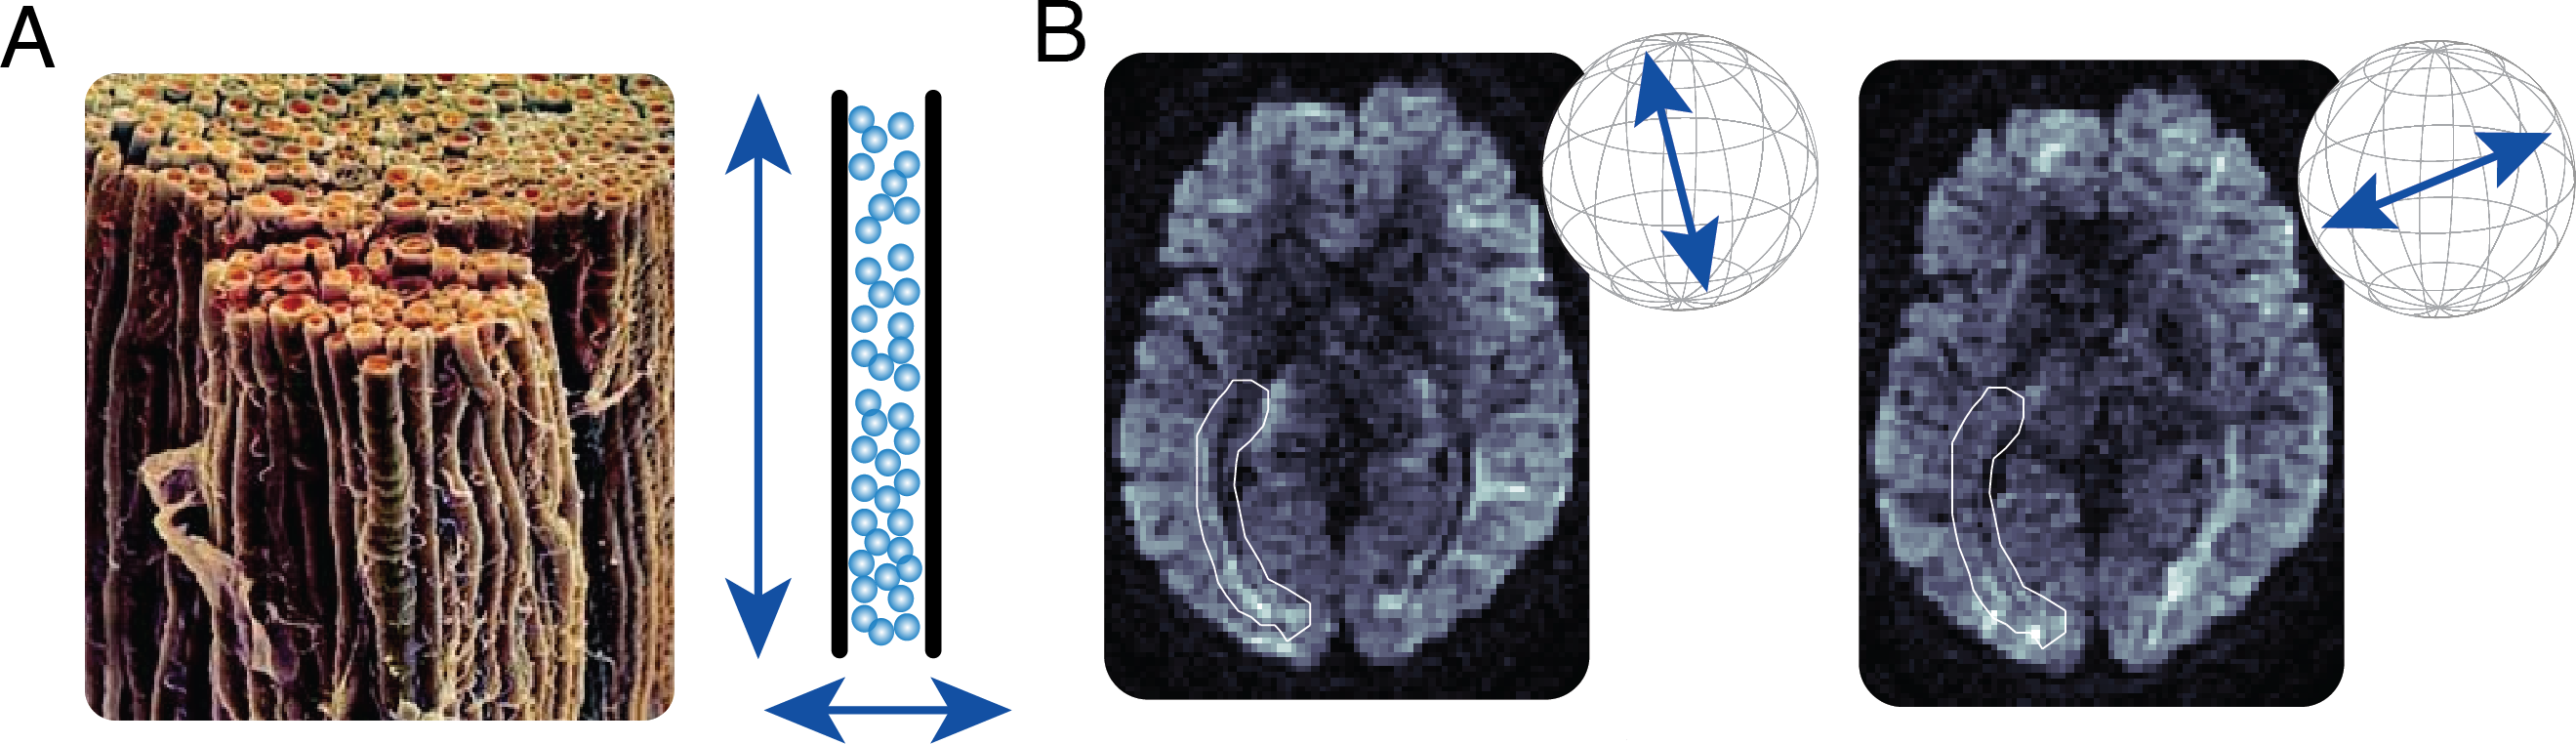
\includegraphics[width=0.77\linewidth]{dti_inference.png}
    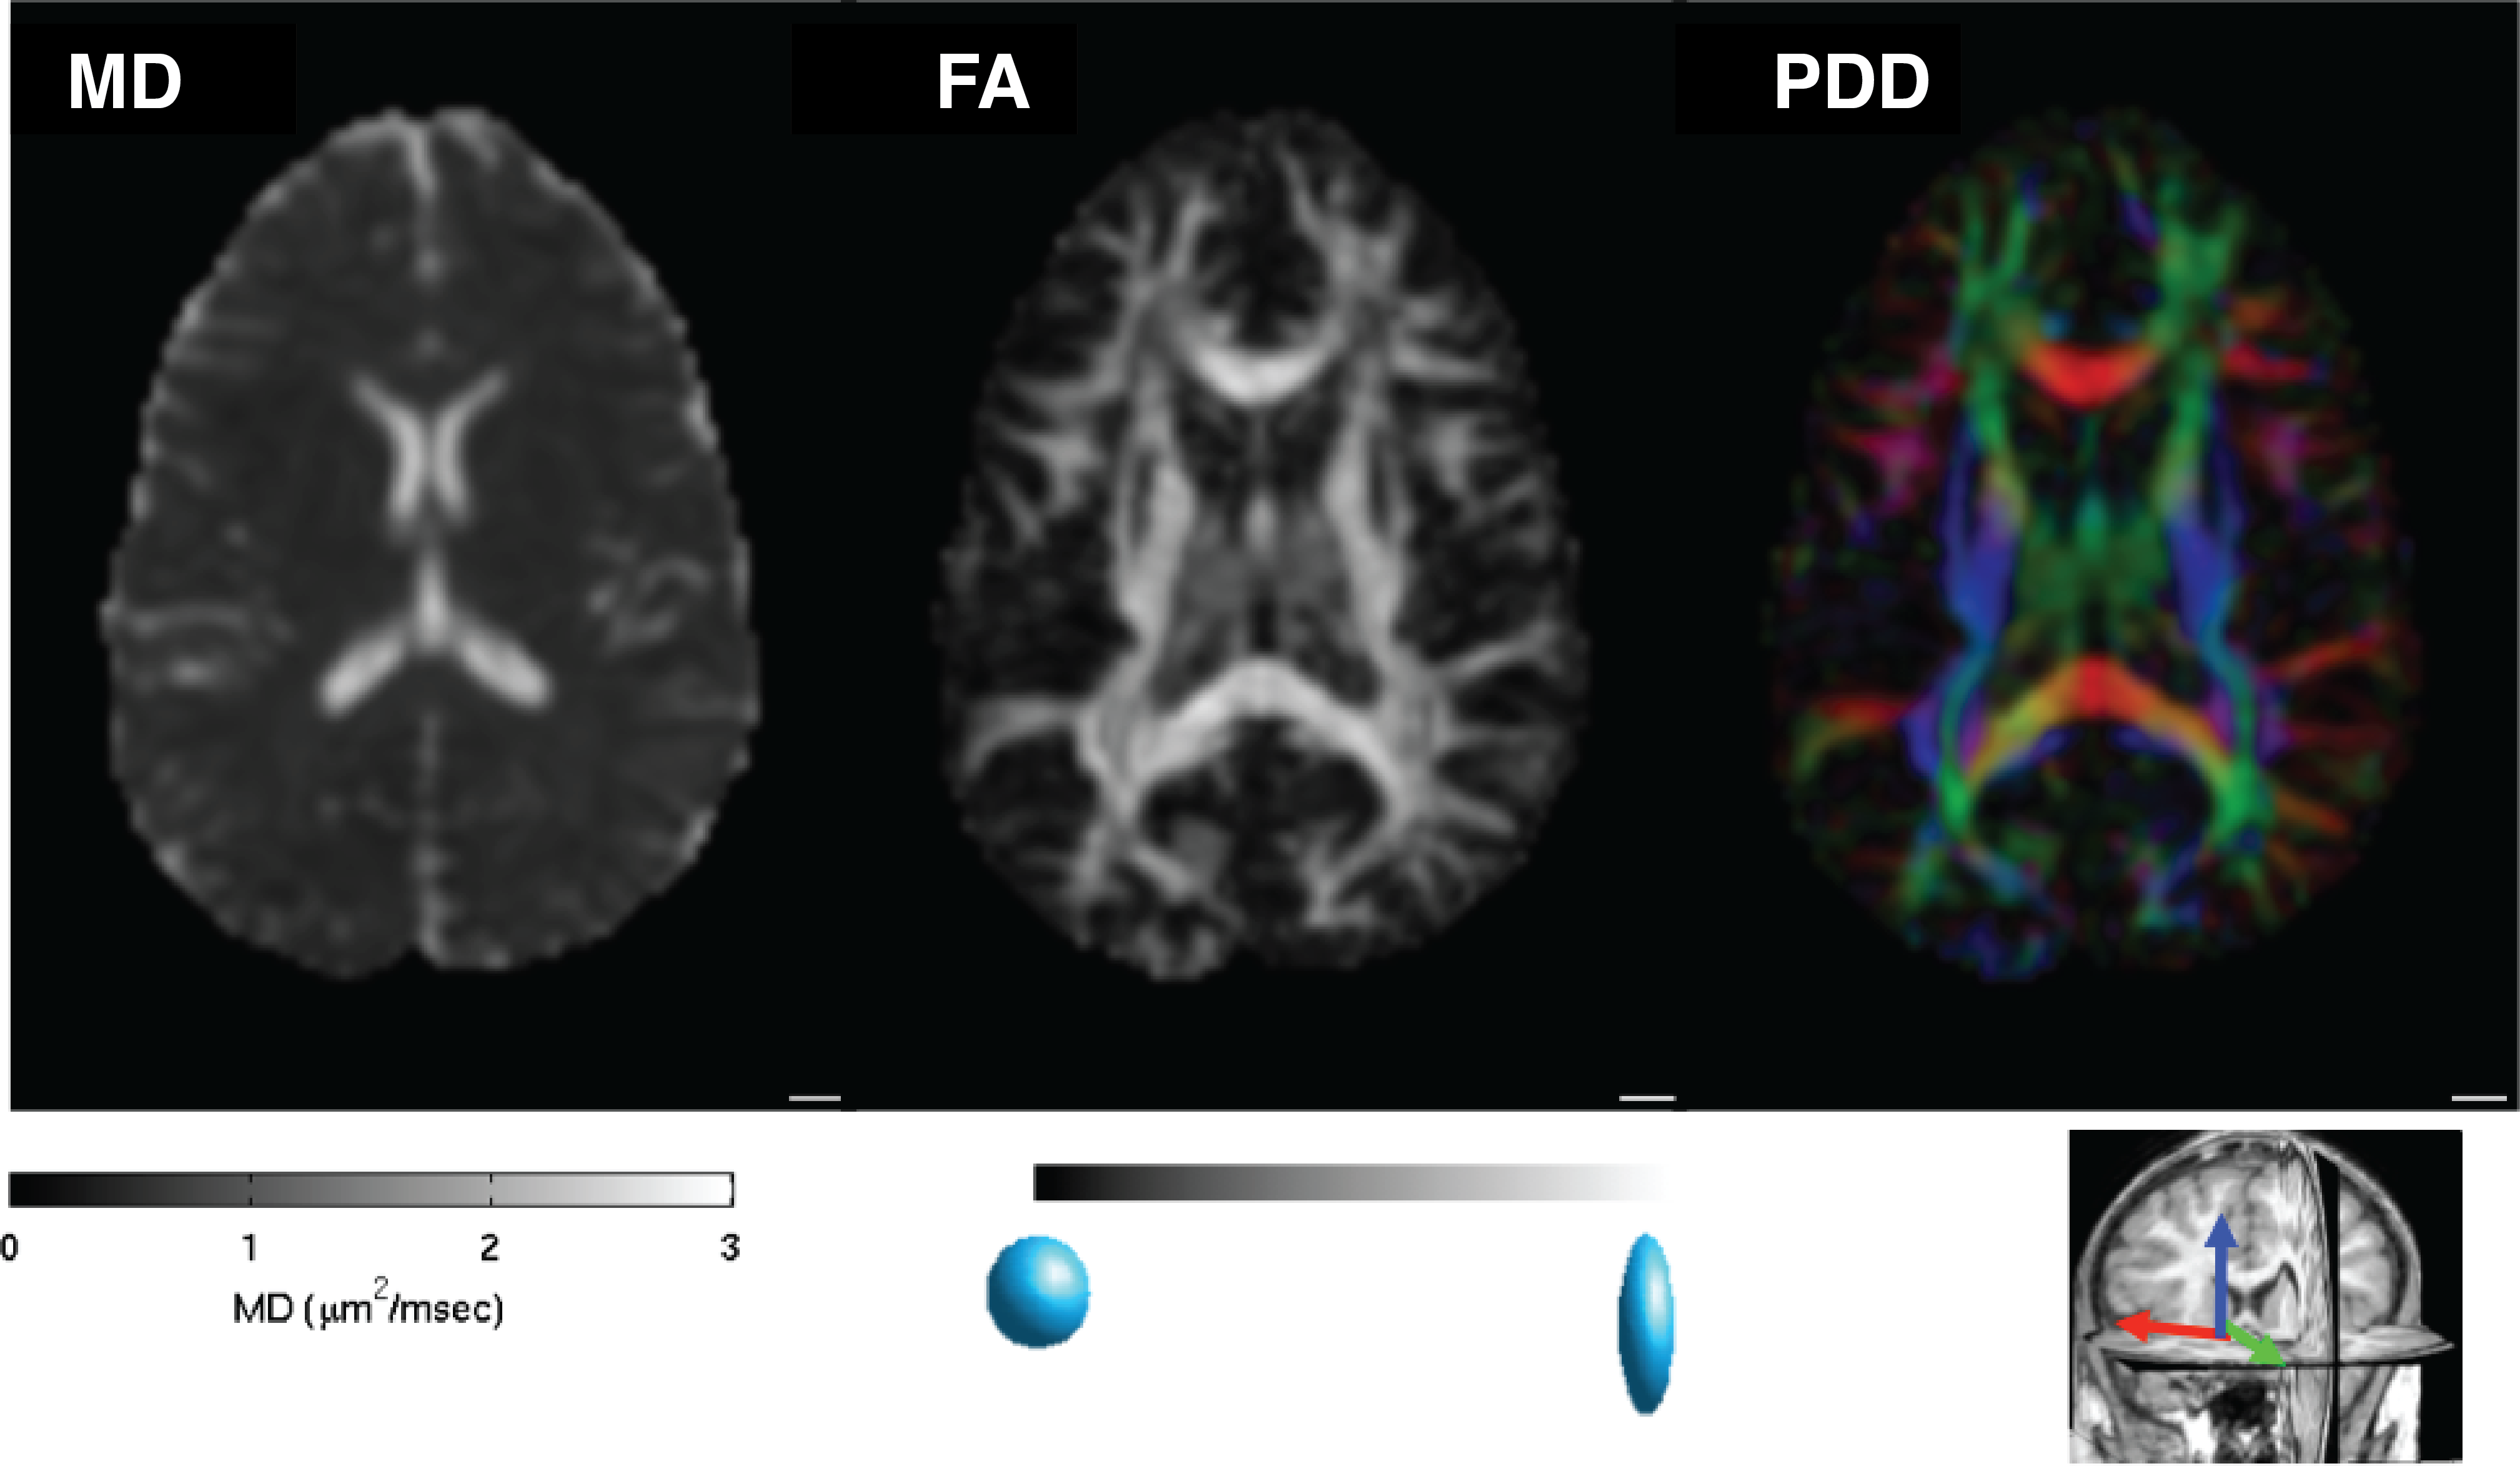
\includegraphics[width=0.77\linewidth]{dti_metrics.png}
    \captionof{figure}{Diffusion Tensor Imaging. \textbf{top}: (\textbf{A}) Human optic nerve next to anisotropic water diffusion. (\textbf{B}) dMRI measurements in a human brain slice, as imaged with two different $\mathbf{b}$-vectors (inset arrows). The image darkens where $\mathbf{b}$-vector aligns with fascicles. \textbf{bottom}: Estimates of white matter organization. MD measures mean diffusion in all directions. FA represents diffusion variability in different directions. The PDD is the direction of maximal diffusion in each voxel. (Rokem et al.~2017)}
\end{Figure}

\noindent Tractometry further reduces the dimensionality of this data by quantifying diffusion metrics along tract profiles.

\begin{Figure}
    \centering
    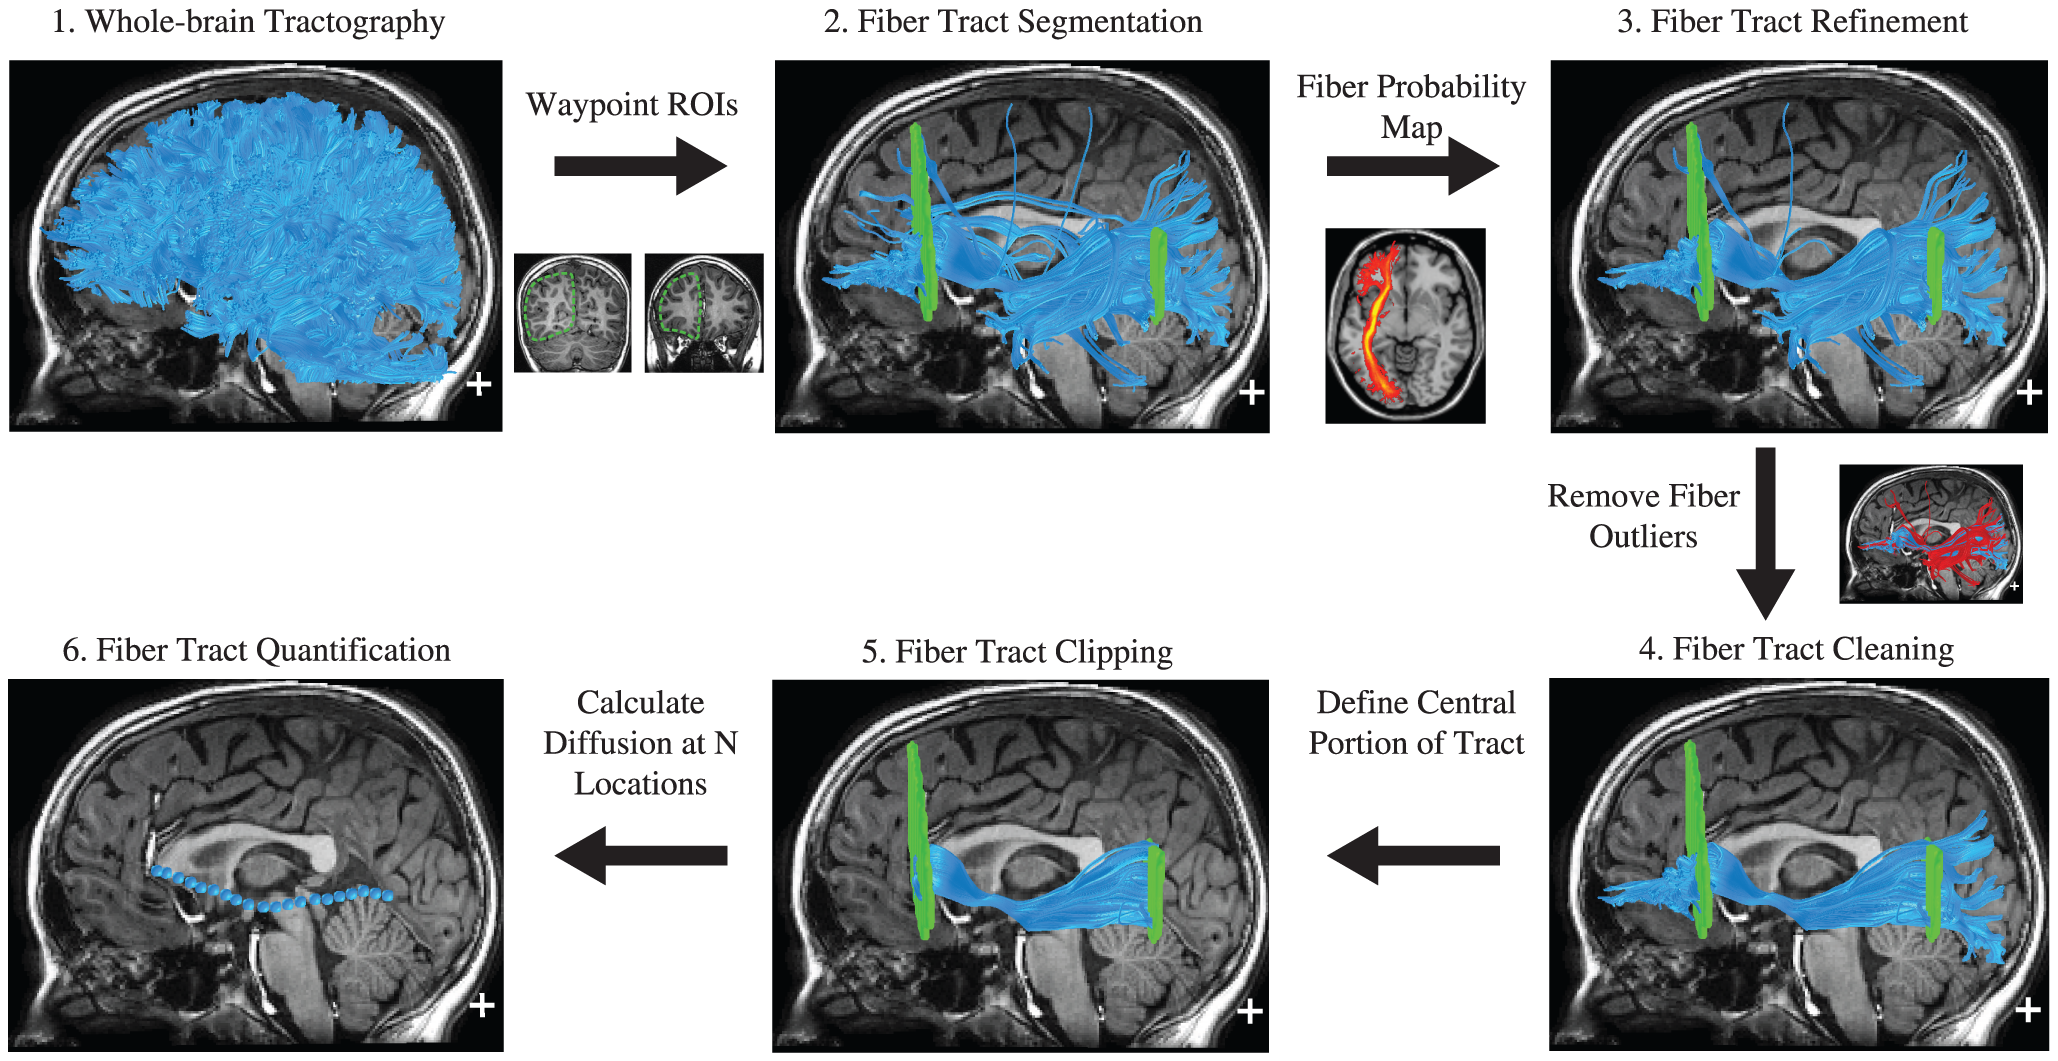
\includegraphics[width=\linewidth]{afq_pipeline.png}
    \captionof{figure}{The preprocessing pipeline: Automated Fiber Quantification (AFQ) identifies fiber tracts, creating tract profiles of common diffusion metrics along canonical white matter tracts (from Yeatman et al.~2012).}
\end{Figure}
}

%----------------------------------------------------------------------------
%	METHODS
%----------------------------------------------------------------------------

\headerbox{Methods}{name=methods,column=0,below=introduction}{

\begin{wrapfigure}[8]{l}{0.43\linewidth}
    \vspace{-1.25em}
    \centering
    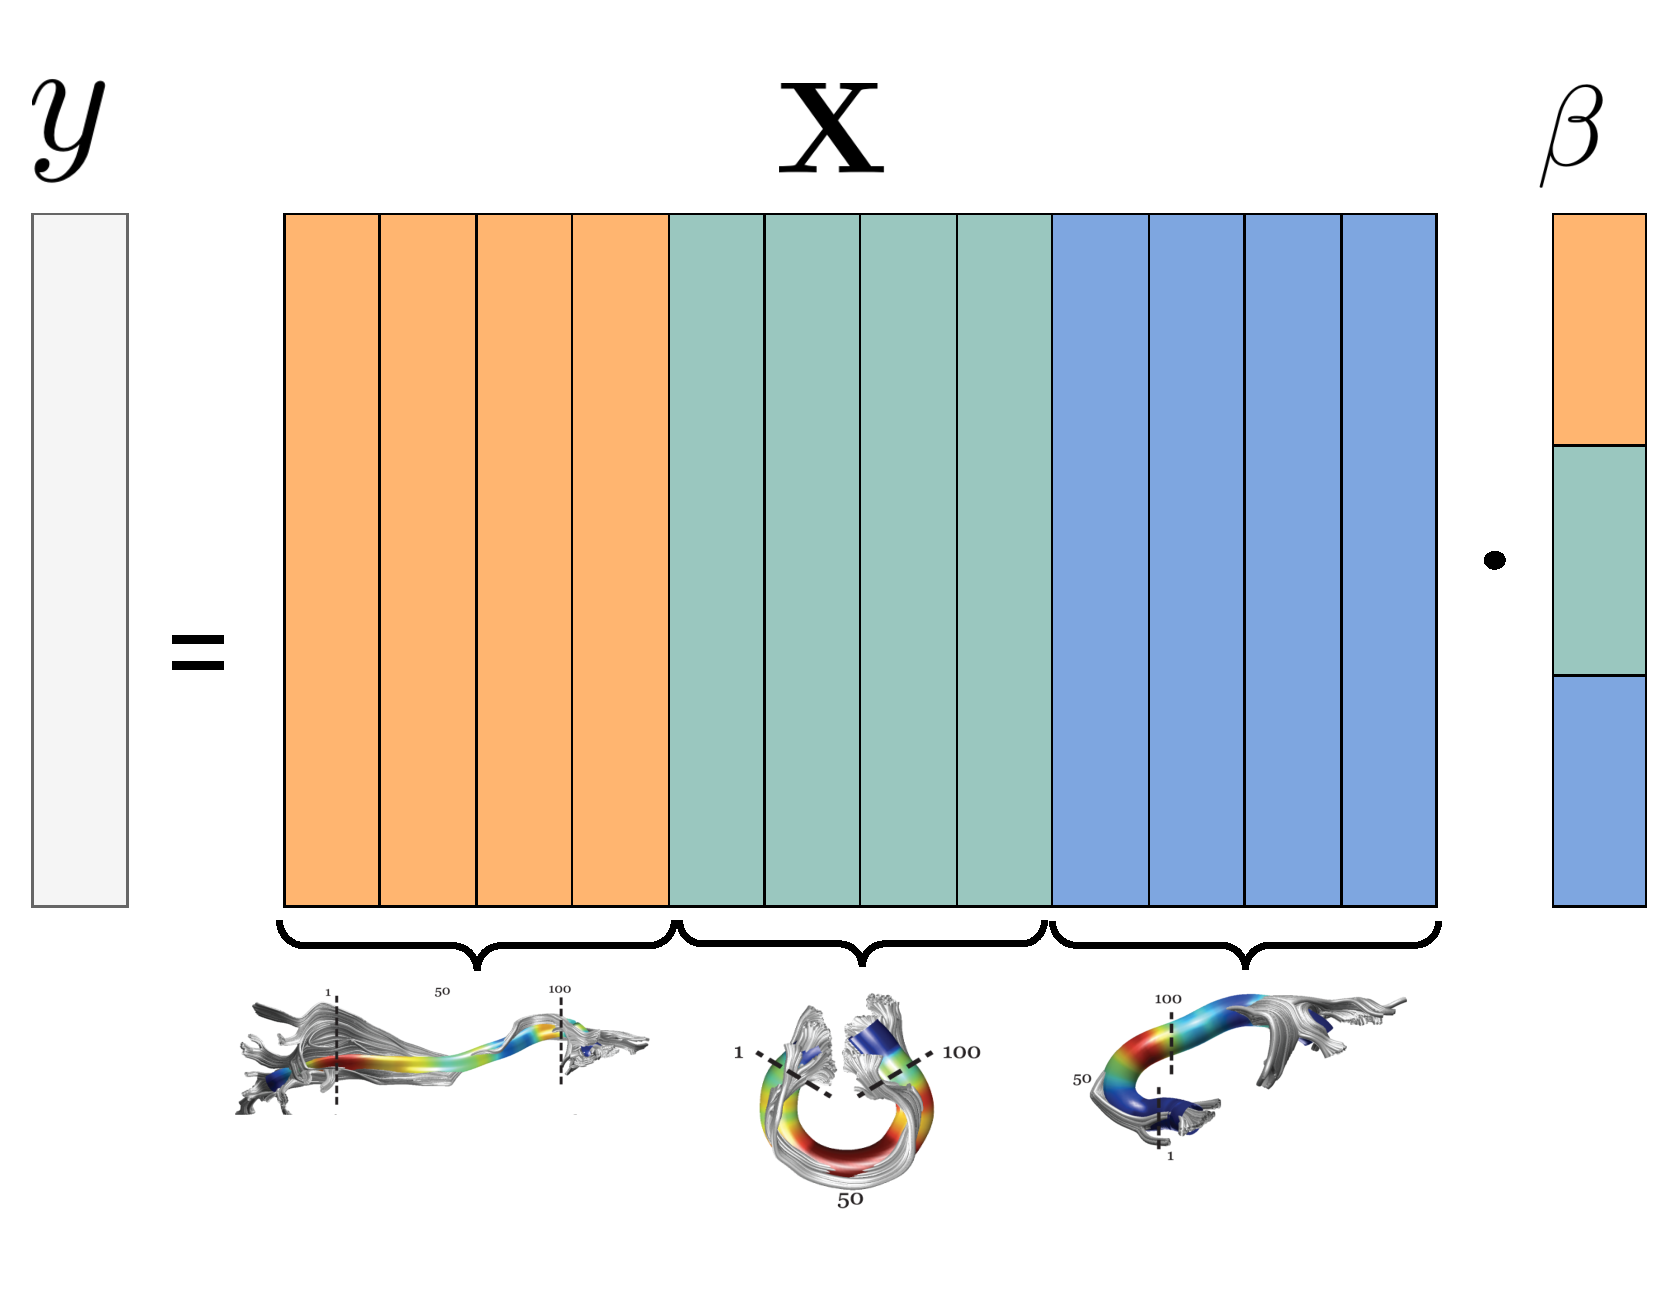
\includegraphics[width=\linewidth]{group_structure.pdf}
    \vspace{-1.25em}
\end{wrapfigure}

\begingroup
\setlength\abovedisplayskip{0.5em}
We use AFQ to generate tractometry data as input to our model and then fit a linear model to the data,
\begin{equation*}
    y = f^{-1} \left( \mathbf{X} \cdot \beta \right),
\end{equation*}
where
\vspace{1em}
\begin{align*}
    y &\coloneqq \text{phenotype} \; (n_\text{subjects} \times 1), \\
    \mathbf{X} &\coloneqq \text{tractometry data} \; (n_\text{subjects} \times n_\text{features}), \\
    \beta &\coloneqq \text{regression coefficients} \; (n_\text{features} \times 1), \\
    f &\coloneqq \text{target transformation function, e.g.} \; f(y) = \log_n(y).
\end{align*}
The feature matrix, $\mathbf{X}$, has inherent group structure, containing groups for each diffusion metric and each fiber bundle.
The high dimensionality of the data ($n_\text{features} \sim \mathcal{O}(10^4)$) requires regularization to avoid overfitting. We use the Sparse Group Lasso (SGL),
\vspace{-0.5em}
\begin{equation*}
    \widehat{\beta} = \min_\beta \Biggl\{
        \underbrace{
            \vphantom{\lambda_1 \displaystyle \sum_\ell \sqrt{p_\ell} \norm{\beta^{(\ell)}}_2}
            \norm{\widehat{y} - \mathbf{X} \cdot \beta}_2^2
        }_{\text{Linear regression}}
        + \underbrace{
            \lambda_1 \displaystyle \sum_\ell \sqrt{p_\ell} \norm{\beta^{(\ell)}}_2
        }_{\text{Group Lasso Penalty}}
        + \underbrace{
            \vphantom{\lambda_1 \displaystyle \sum_\ell \sqrt{p_\ell} \norm{\beta^{(\ell)}}_2}
            \lambda_2 \norm{\beta}_1
        }_{\text{Lasso Penalty}}
    \Biggl\}
\end{equation*}
SGL enforces sparsity at both the \textbf{inter}-group level (using $\lambda_1$) and \textbf{intra}-group level (using $\lambda_2$). The hyperparameters $\lambda_1, \lambda_2, n$ are optimized through nested $k$-fold cross-validation.
\endgroup
}

%----------------------------------------------------------------------------
%	CONCLUSION
%----------------------------------------------------------------------------

\headerbox{Conclusion}{name=conclusion,column=0,below=methods}{

\begin{itemize}[nosep, leftmargin=*]
\item Novel method for analysis of dMRI tractometry data

    \begin{itemize}[nosep, leftmargin=*]
    \item Accurate prediction of phenotypic information
    \item Interpretable results and identification of important features
    \end{itemize}

\item Applicable to both localized and global phenomena
\item Packaged as open-source software called AFQ-Insight: \texttt{https://github.com/richford/AFQ-Insight}

\item Integrates into broader AFQ software ecosystem:
    \begin{itemize}[nosep, leftmargin=*]
    \item pyAFQ: produces input tractometry data from raw dMRI
    \item AFQ-Browser: visualization, analysis, and sharing of dMRI studies
    \end{itemize}
\end{itemize}
}

%----------------------------------------------------------------------------
%	ACKNOWLEDGEMENTS
%----------------------------------------------------------------------------

\headerbox{Acknowledgements}{name=acknowledgements,column=0,below=conclusion,above=bottom}{

\smaller % Reduce the font size in this block

\includegraphics[height=0.88cm]{SloanLogo.png}

\includegraphics[height=0.88cm]{MooreFdn.png}

\includegraphics[height=0.88cm]{eSciencelogo.png}
}

%----------------------------------------------------------------------------
%	RESULTS 1
%----------------------------------------------------------------------------

\headerbox{Results: Classifying Patients with ALS}{name=results1,span=2,column=1,row=0}{ % To reduce this block to 1 column width, remove 'span=2'

\begin{itemize}[noitemsep, leftmargin=*]
    \item Previous study measured dMRI in patients with amyotrophic lateral sclerosis (ALS) (Sarica et al.~2017).
    \begin{itemize}[noitemsep, leftmargin=*]
        \item 24 ALS patients and 24 demographically matched controls
        \item Previous state of the art achieved 80\% accuracy using random forests and \emph{a priori} feature selection.
    \end{itemize}
    \item Our method outperforms previous results, with an accuracy of 93$\pm$2\% and an area under the ROC curve of 0.978$\pm$0.006.
\end{itemize}
\begin{Figure}
    \centering
    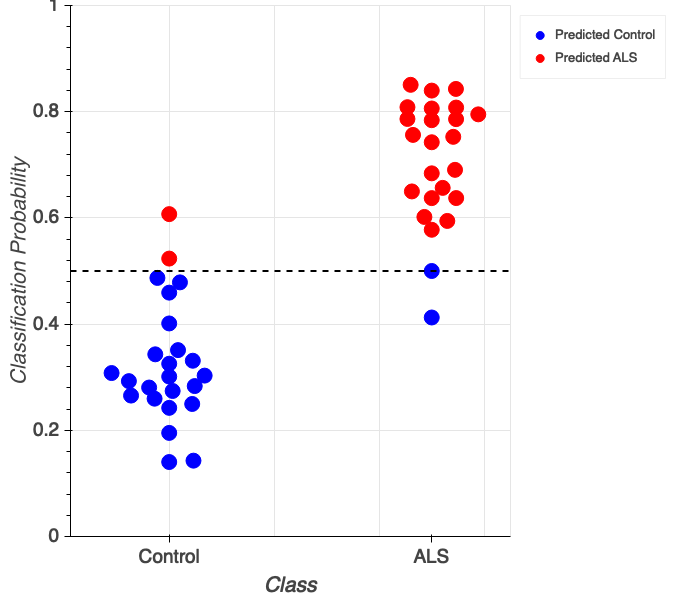
\includegraphics[height=0.28\linewidth, valign=t]{classification_probs.png}
    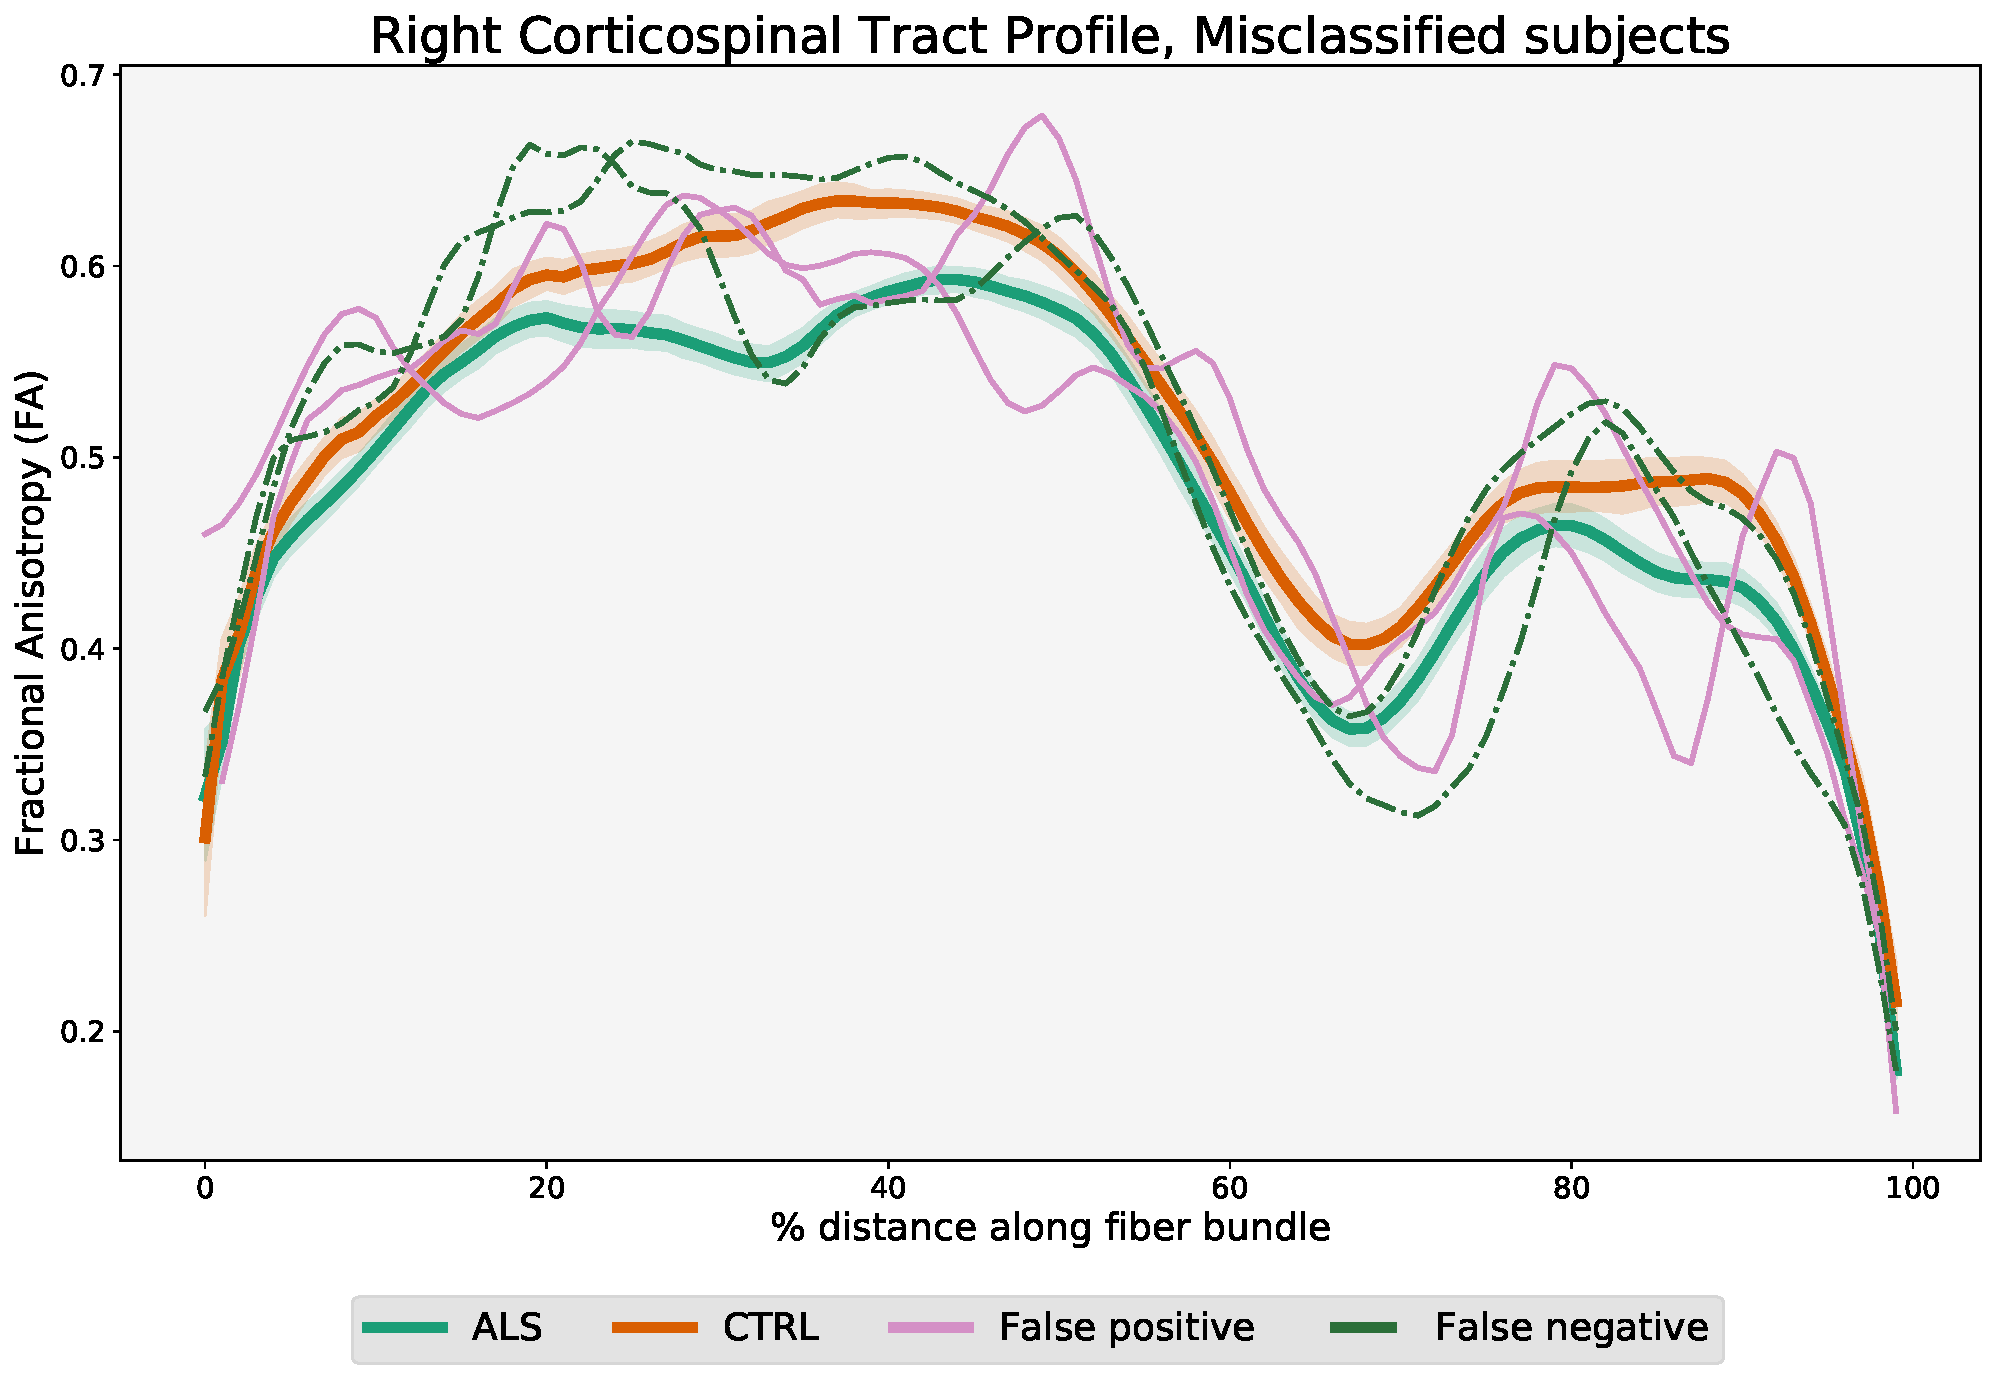
\includegraphics[height=0.28\linewidth, valign=t]{classification_subjects_profiles.pdf}
    \captionof{figure}{\textbf{left}: Classification probabilities for each subject's ALS diagnosis. Controls are on the left while subjects with ALS are on the right. Predicted controls are in blue and predicted patients are in red. Thus false positives are represented as red dots on the left while false negatives are represented as blue dots on the right. \textbf{right}: The tract profiles of the misclassified subjects suggest that they are justifiably hard to classify.}
\end{Figure}
\begin{itemize}[noitemsep, leftmargin=*]
\item Moreover, it automatically identifies the corticospinal tract (CST) as the critical feature for differentiating patients with ALS from controls
\item Thus, well-known features of the disease can be recovered through an automated, data-driven approach.
\end{itemize}
\begin{Figure}
    \centering
    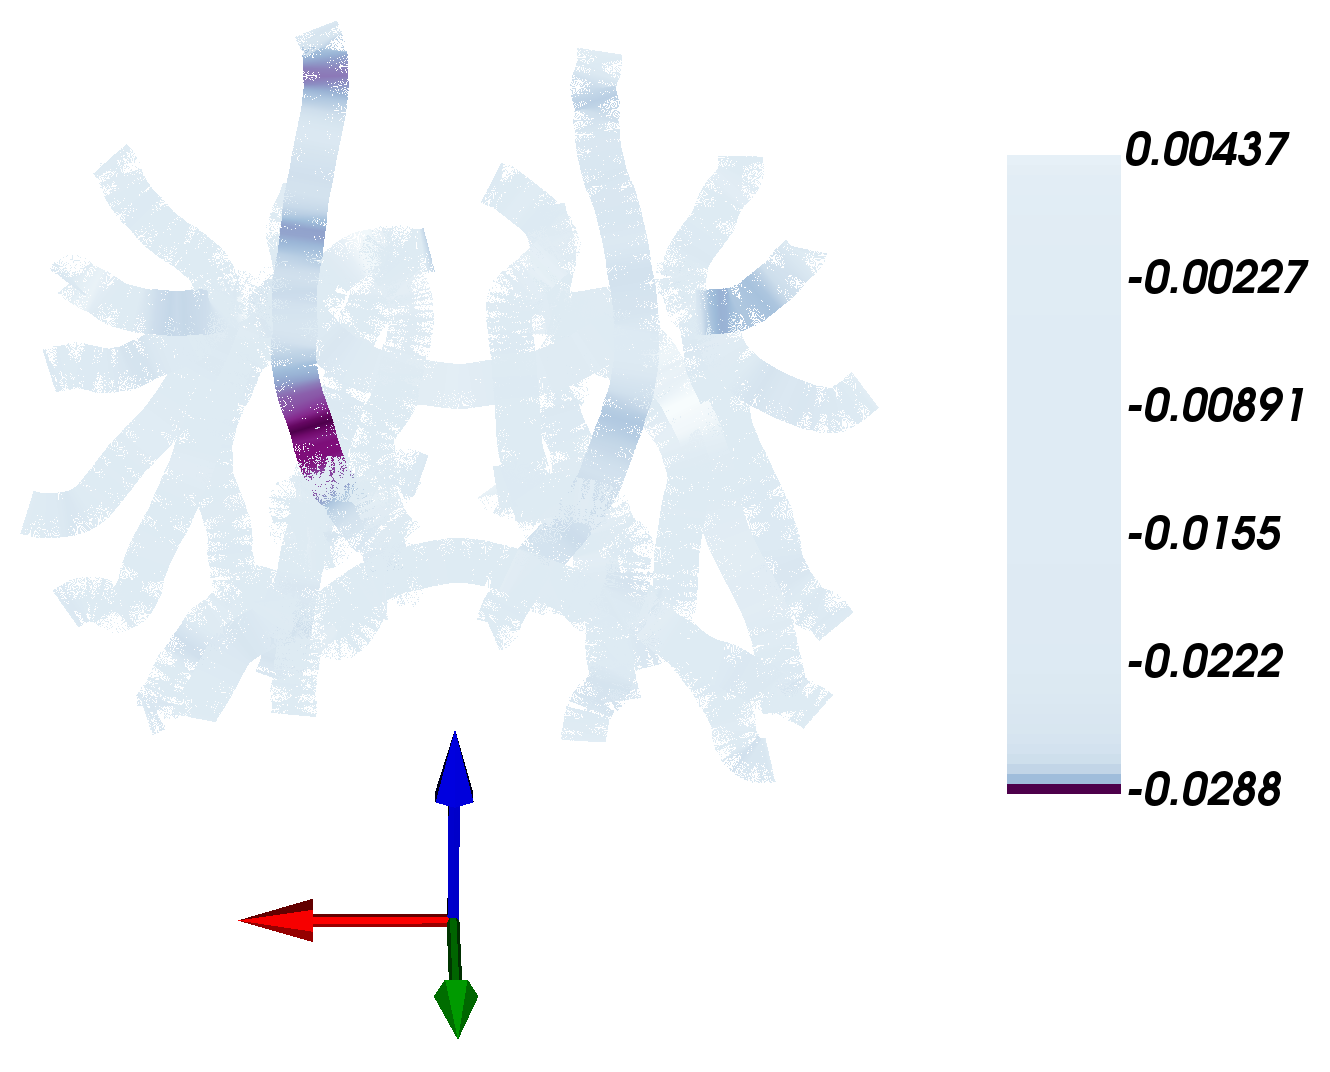
\includegraphics[height=0.28\linewidth, valign=t]{classification_beta_bupu.png}
    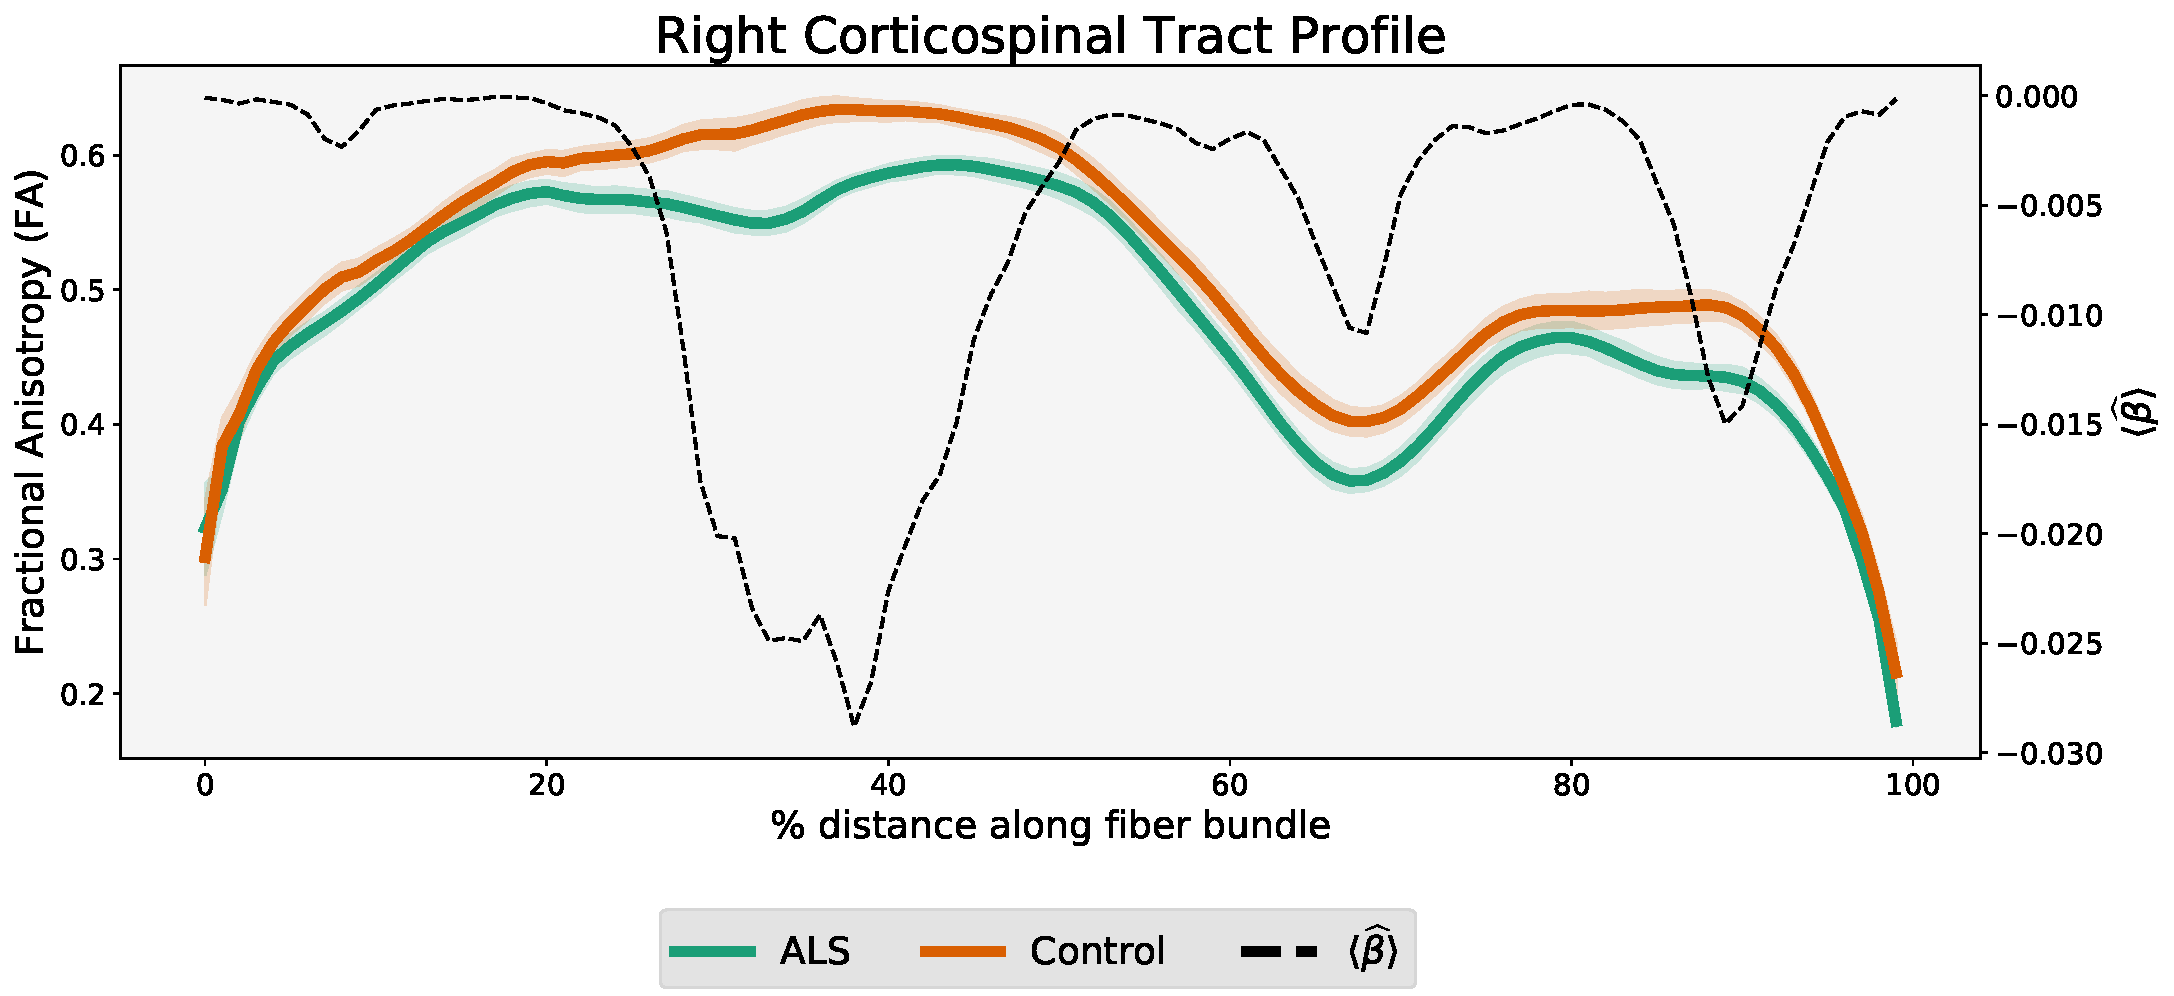
\includegraphics[height=0.28\linewidth, valign=t]{classification_tract_profiles.pdf}
    \captionof{figure}{Classification feature importance: \textbf{left}: $\widehat{\beta}$ for the FA metric, represented along the ``core fibers'' for each tract. The feature importance is sparse and dominated by the right CST. \textbf{right}: The FA tract profiles for the right CST, grouped by ALS class and the mean $\widehat{\beta}$ (dotted, black). Larger $\widehat{\beta}$ values indicate areas of distinction between patients with ALS and controls.}
\end{Figure}
}

%----------------------------------------------------------------------------
%	RESULTS 2
%----------------------------------------------------------------------------

\headerbox{Results: Predicting ``Brain Age''}{name=results2,span=2,column=1,below=results1}{ % To reduce this block to 1 column width, remove 'span=2'

\begin{minipage}[t]{0.45\linewidth}
\vspace{1em}
\noindent In a regression setting, data from a previous study (Yeatman et al.~2014) can be used to predict ``brain age.''
\begin{itemize}
    \item 77 subjects with ages 6-50.
    \item We predict subjects' chronological age with a median absolute error of 3.6 yrs and $R^2 \approx 0.3$.
    \item Older subjects have higher residual variance, reflecting the automatically-chosen log-transformation and implying that brain age becomes more difficult to predict as we age chronologically.
    \item In contrast to the ALS classification case, brain age feature importance is dense and non-localized.
\end{itemize}
\end{minipage}
\hspace{0.03\linewidth}
\begin{minipage}[t]{0.5\linewidth}
\begin{Figure}
    \centering
    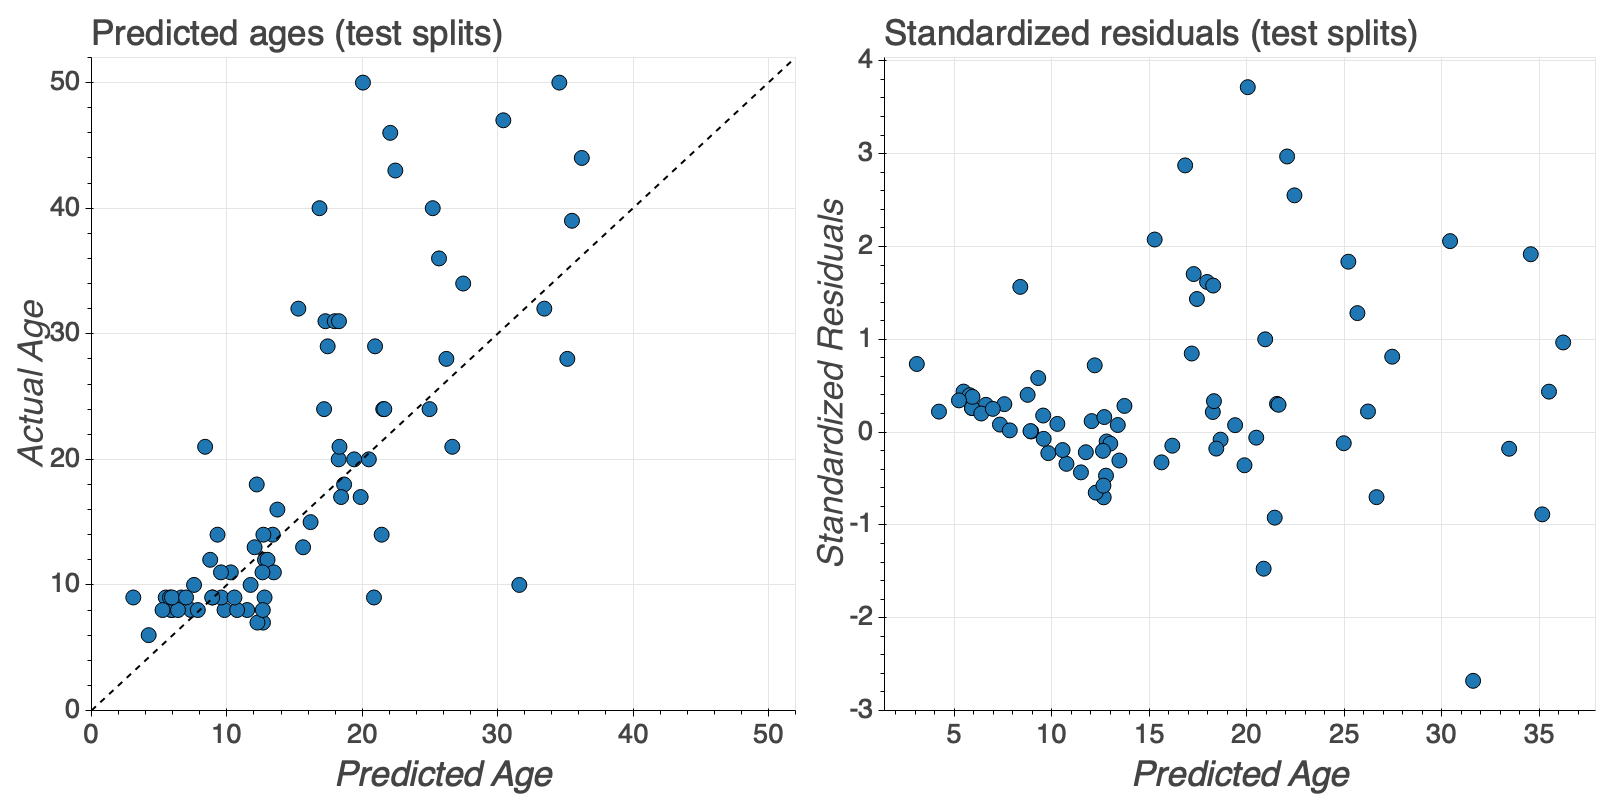
\includegraphics[width=\linewidth]{regression_residuals.png}
    \captionof{figure}{Regression results: \textbf{left}: Predicted age vs. actual age. SGL achieves a median absolute error of 3.6 years with an $R^2$ of $\sim0.3$. \textbf{right}: Predicted age vs.~standardized residuals for age regression.}
\end{Figure}
\end{minipage}

\begin{Figure}
    \centering
    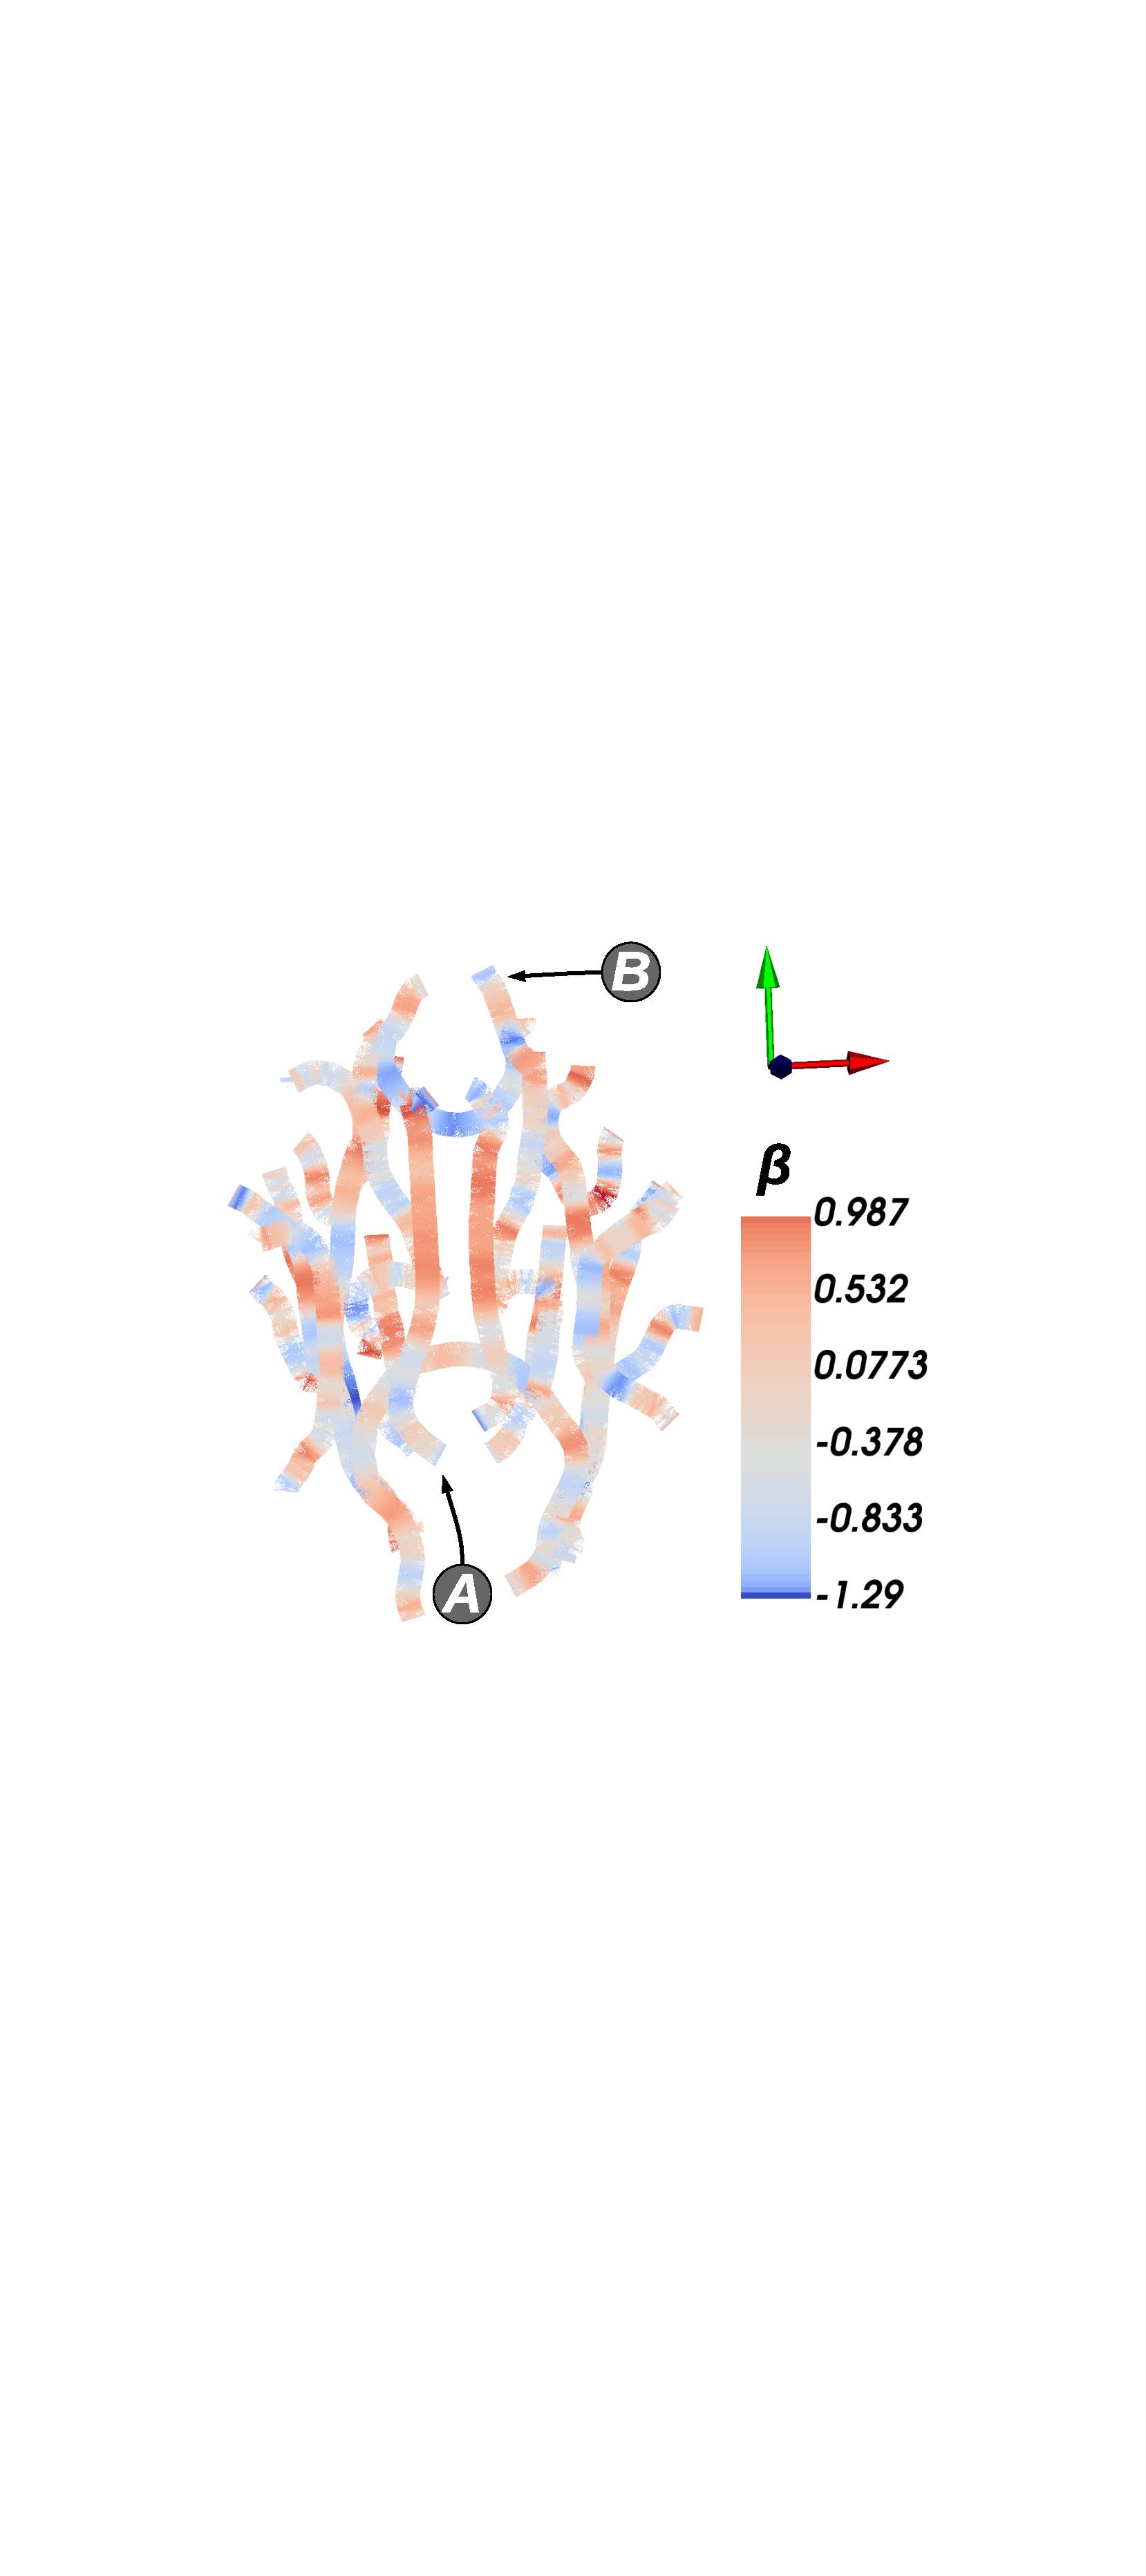
\includegraphics[height=0.28\linewidth, valign=t]{regression_beta_annotated.pdf}
    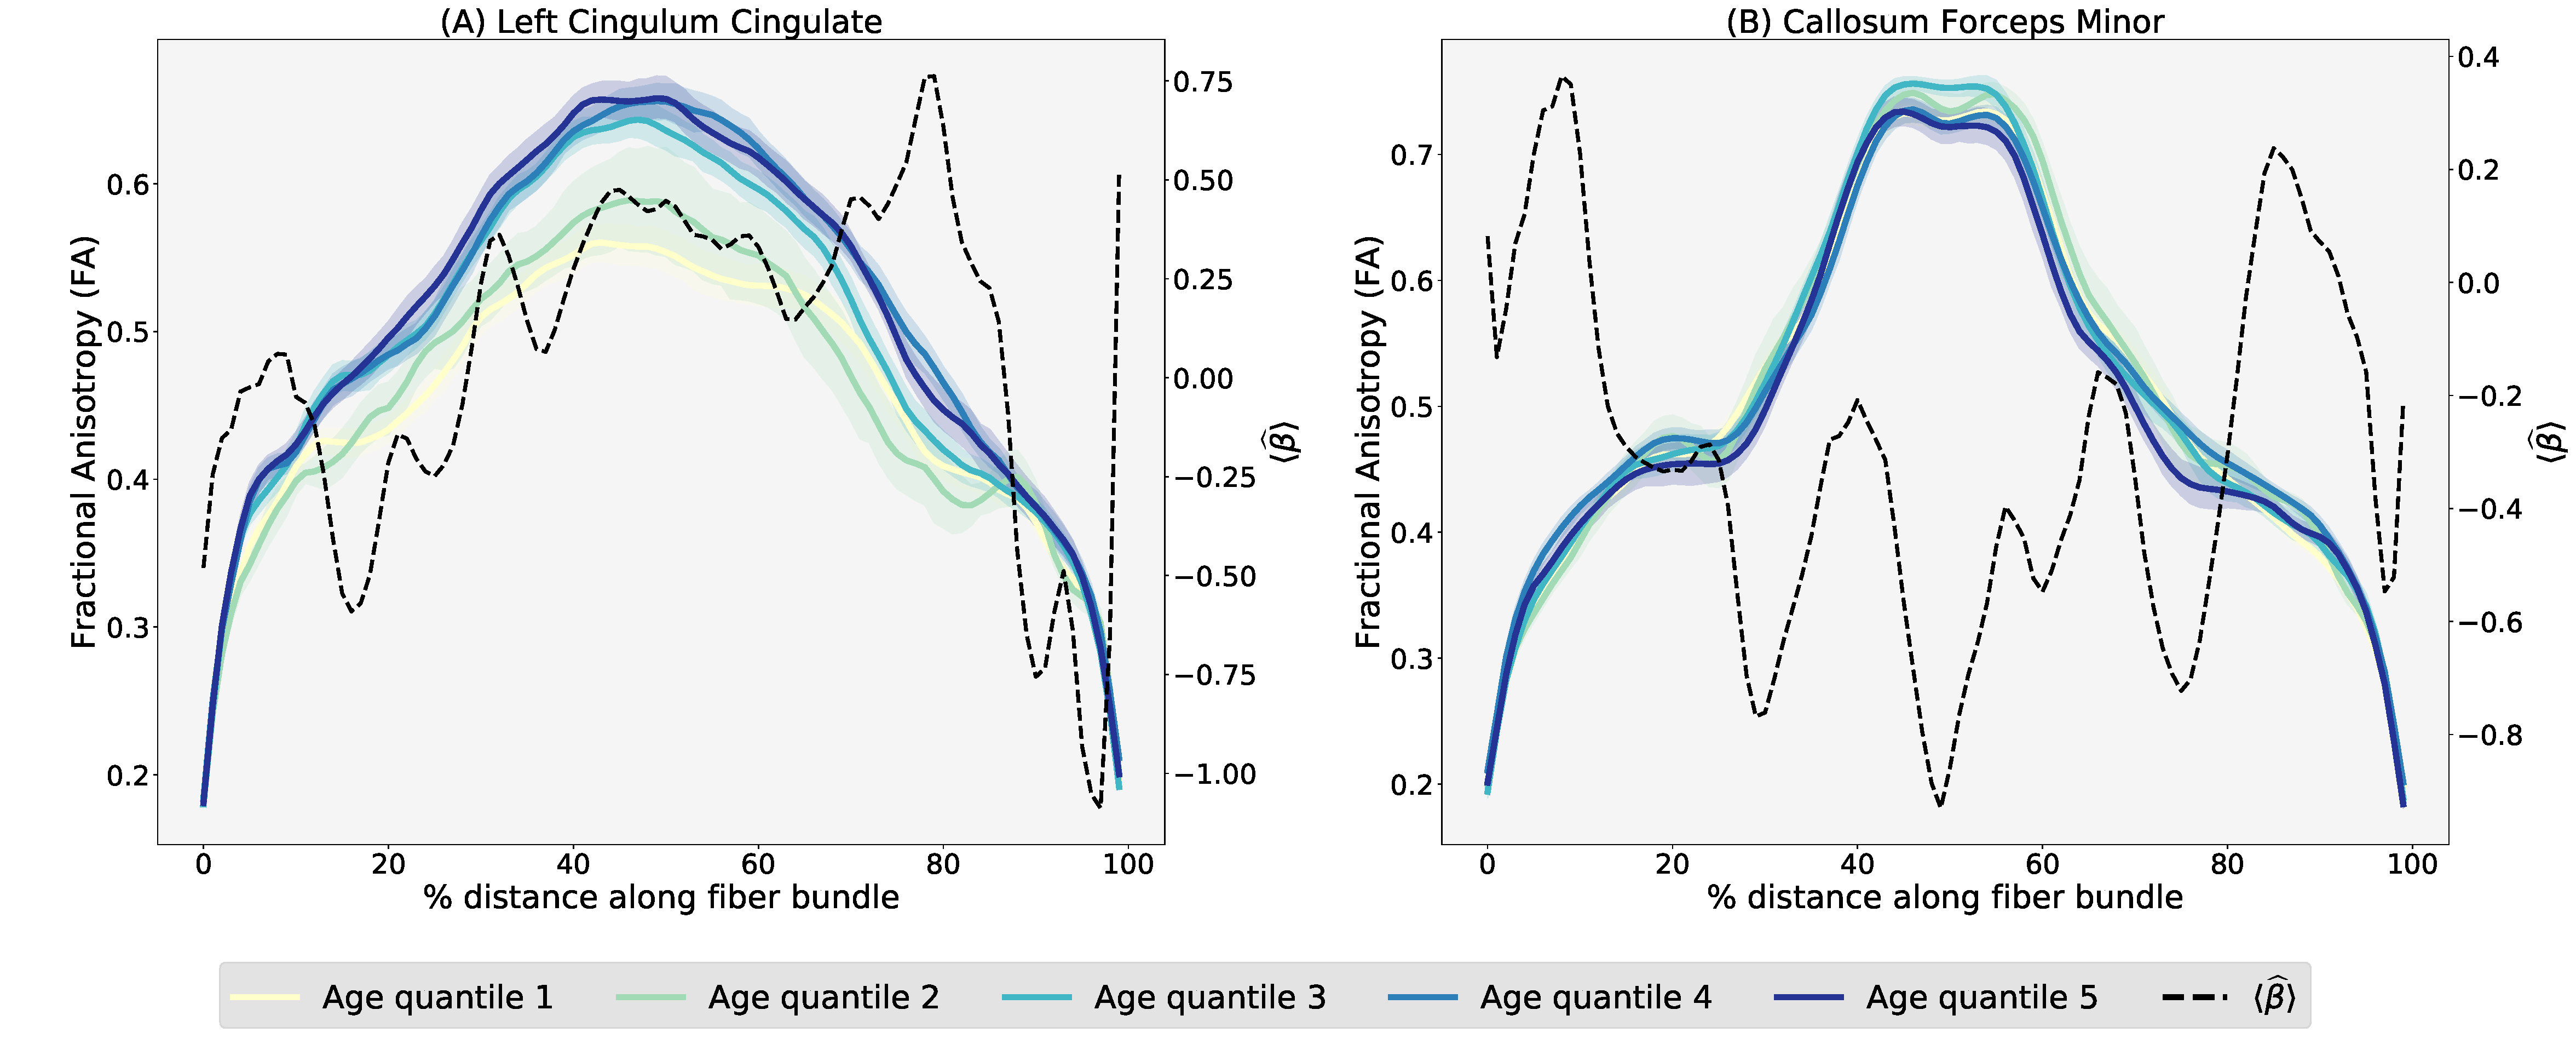
\includegraphics[height=0.28\linewidth, valign=t]{regression_tract_profiles.pdf}
    \captionof{figure}{Regression feature importance: \textbf{left}: $\widehat{\beta}$ for the FA metric, represented along the ``core fibers'' for each tract. Red indicates positive correlation with age while blue indicates negative correlation. \textbf{middle \& right}: The FA tract profiles for the Left Cingulum Cingulate and Callosum Forceps Minor, grouped by age quintile (color) and the mean $\widehat{\beta}$ (dotted, black). Larger $\widehat{\beta}$ values indicate areas of distinction between age quintile.}
\end{Figure}
}

%----------------------------------------------------------------------------
%   REFERENCES
%----------------------------------------------------------------------------

\headerbox{References}{name=references,span=2,column=1,below=results2,above=bottom}{

\begin{multicols}{2}
\smaller \smaller % Reduce the font size in this block
\renewcommand{\section}[2]{\vskip 0.05em} % Get rid of the default "References" section title
\nocite{*} % Insert publications even if they are not cited in the poster

\bibliographystyle{unsrt}
\bibliography{poster}
\end{multicols}
}

\end{poster}

\end{document}
